% Created 2022-03-10 Thu 14:35
% Intended LaTeX compiler: pdflatex
\documentclass[presentation,aspectratio=169, usenames, dvipsnames]{beamer}
\usepackage[utf8]{inputenc}
\usepackage[T1]{fontenc}
\usepackage{graphicx}
\usepackage{grffile}
\usepackage{longtable}
\usepackage{wrapfig}
\usepackage{rotating}
\usepackage[normalem]{ulem}
\usepackage{amsmath}
\usepackage{textcomp}
\usepackage{amssymb}
\usepackage{capt-of}
\usepackage{hyperref}
\usepackage{khpreamble}
\usepackage{amssymb}
\usepgfplotslibrary{groupplots}
\newcommand*{\shift}{\operatorname{q}}
\definecolor{ppc}{rgb}{0.1,0.1,0.6}
\definecolor{iic}{rgb}{0.6,0.1,0.1}
\definecolor{ddc}{rgb}{0.1,0.6,0.1}
\DeclareMathSymbol{\Omega}{\mathalpha}{letters}{"0A}% italics
\DeclareMathSymbol{\varOmega}{\mathalpha}{operators}{"0A}% upright
\providecommand*{\upOmega}{\varOmega}% for siunitx
\usepackage[binary-units=true]{siunitx}
\usetheme{default}
\author{Kjartan Halvorsen}
\date{2021-03-08}
\title{Control PID}
\hypersetup{
 pdfauthor={Kjartan Halvorsen},
 pdftitle={Control PID},
 pdfkeywords={},
 pdfsubject={},
 pdfcreator={Emacs 26.3 (Org mode 9.4.6)}, 
 pdflang={English}}
\begin{document}

\maketitle

\section{PID parameter intuition}
\label{sec:org72574f0}

\begin{frame}[label={sec:org244dff4}]{Control en lazo cerrado}
   \begin{center}
   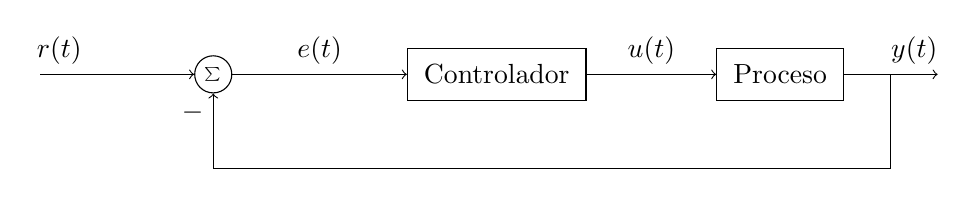
\begin{tikzpicture}[node distance=22mm, block/.style={rectangle, draw, minimum width=15mm, inner sep=6pt}, sumnode/.style={circle, draw, inner sep=2pt}]
  { 
  \node[coordinate] (input) {};
  \node[sumnode, right of=input] (sum) {\tiny $\sum$};
  \node[block, right of=sum, node distance=3.6cm] (reg) {Controlador};
  \node[block, right of=reg, node distance=3.6cm] (plant) {Proceso};
  \node[coordinate, right of=plant, node distance=2cm] (output) {};
  \node[coordinate, below of=plant, node distance=12mm] (feedback) {};
 
  \draw[->] (plant) -- node[coordinate, inner sep=0pt] (meas) {} node[near end, above] {$y(t)$} (output);
  \draw[->] (meas) |- (feedback) -| node[very near end, left] {$-$} (sum);
  \draw[->] (input) -- node[very near start, above] {$r(t)$} (sum);
  \draw[->] (sum) -- node[above] {$e(t)$} (reg);
  \draw[->] (reg) -- node[above] {$u(t)$}(plant);
}
\end{tikzpicture}
\end{center}
\end{frame}


\begin{frame}[label={sec:orgd812958}]{Control en cascada}
\begin{center}
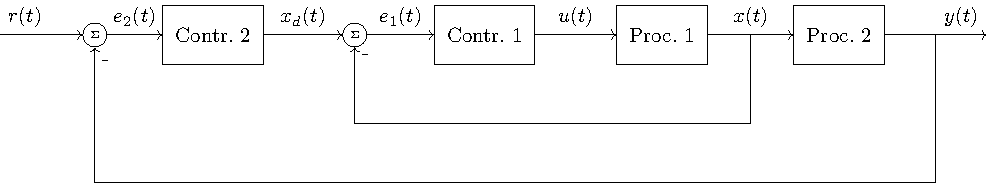
\includegraphics[width=\linewidth]{../../figures/block-diagram-cascade-control.pdf}
\end{center}

\alert{Idea clave} Mejorar el control utilizando más información 
\end{frame}

\begin{frame}[label={sec:orge3d7eb0}]{El controlador PID}
\begin{center}
  \begin{tikzpicture}[node distance=22mm, block/.style={rectangle, draw, minimum width=15mm}, sumnode/.style={circle, draw, inner sep=2pt},scale=0.8, every node/.style={scale=0.8}]

    \node[coordinate] (input) {};
    \node[sumnode, right of=input, node distance=16mm] (sum) {\tiny $\Sigma$};
    \node[block, right of=sum, node distance=20mm] (pid)  {\textcolor{ppc}{P}\textcolor{iic}{I}\textcolor{ddc}{D}};
    \node[coordinate, below of=sum, node distance=12mm] (feedback) {};
    \node[coordinate, right of=pid, node distance=20mm] (output) {};

    \draw[->] (input) -- node[above, pos=0.3] {$r(t)$} (sum);
    \draw[->] (sum) -- node[above] {$e(t)$} (pid);
    \draw[->] (pid) -- node[above, near end] {$u(t)$} (output);
    \draw[->] (feedback) -- node[left, near start] {$y(t)$} node[right, pos=0.95] {-} (sum);

    \begin{scope}[yshift=-3cm]
    \foreach \pos/\clr/\nme in {0/ppc/P, 2/iic/I, 4/ddc/D} {
    \node (knob) at (\pos,0) {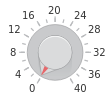
\includegraphics[width=12mm]{../../figures/knob.png}};
    \node[above of=knob, node distance=10mm] {\large \textcolor{\clr}{\nme}};
    }
    \end{scope}

    \end{tikzpicture}
\end{center}

\begin{tabular}{lll}
\textbf{\textcolor{ppc}{P}} & Proporcional: & Controla rapidez de la respuesta\\
\textbf{\textcolor{iic}{I}} & Integral: & Elimina el error $e(t)$ en estado estable\\
\textbf{\textcolor{ddc}{D}} & Derivada: & Da amortiguación
\end{tabular}
\end{frame}

\begin{frame}[label={sec:org730c919}]{El controlador PID}
\begin{columns}
\begin{column}{0.6\columnwidth}
\begin{center}
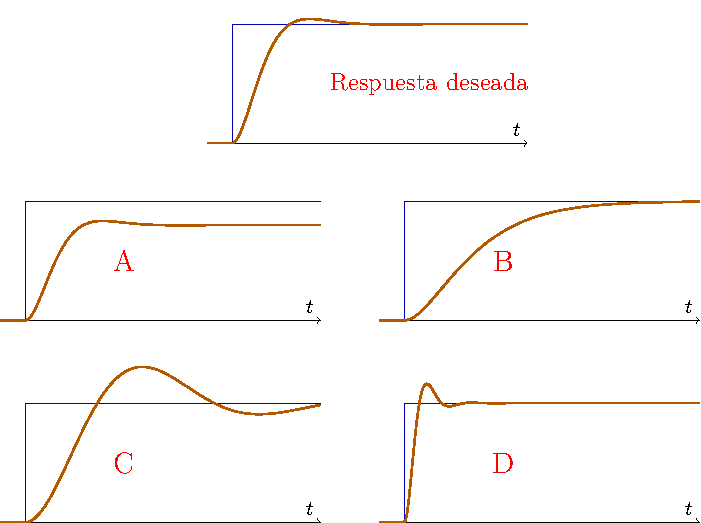
\includegraphics[width=0.99\linewidth]{../../figures/stepresponse-secondorder-exercise}
\end{center}
\end{column}

\begin{column}{0.4\columnwidth}
\alert{Actividad} Cómo ajustar las ganancias P, I y D para obtener la respuesta deseada?

\begin{center}
\begin{tabular}{llll}
Caso & \textcolor{ppc}{P} & \textcolor{iic}{I} & \textcolor{ddc}{D}\\
\hline
A &  &  & \\
B &  &  & \\
C &  &  & \\
D &  &  & \\
\hline
\end{tabular}
\end{center}
\end{column}
\end{columns}
\end{frame}

\begin{frame}[label={sec:org6fd989f}]{El controlador PID en forma paralela}
\begin{center}
  \begin{tikzpicture}[node distance=22mm, block/.style={rectangle, draw, minimum width=12mm}, sumnode/.style={circle, draw, inner sep=2pt},
  amp/.style = {regular polygon, regular polygon sides=3,
           draw, fill=white, text width=1em,
           inner sep=1pt, outer sep=0mm,
           shape border rotate=-90},
     ]

    \node[coordinate] (input) {};
    \node[sumnode, right of=input, node distance=16mm] (sum) {\tiny $\Sigma$};
    \node[color=iic, amp, right of=sum, node distance=28mm, inner sep=0pt] (ig)  {$\frac{1}{\tau_i}$};
    \node[color=iic,block, right of=ig, node distance=18mm] (ii)  {$\int$};
    \node[color=ppc, coordinate, above of=ii, node distance=10mm] (pp)  {};
    \draw[->, color=iic] (ig)  -- node[coordinate,] (mp) {} (ii);
    \node[color=ddc, amp, below of=mp, node distance=14mm] (dg)  {$\tau_d$};
    \node[color=ddc,block, right of=dg, node distance=18mm] (dd)  {$\frac{d}{dt}$};
    \node[sumnode, right of=ii, node distance=20mm] (sum2) {\tiny $\Sigma$};
    \node[amp, right of=sum2, node distance=20mm] (gain)  {$k_c$};
    \node[coordinate, below of=sum, node distance=12mm] (feedback) {};
    \node[coordinate, right of=gain, node distance=20mm] (output) {};

    \draw[->] (input) -- node[above, pos=0.3] {$r(t)$} (sum);
    \draw[->] (sum) -- node[above, pos=0.2] {$e(t)$} node[coordinate] (mm) {}  (ig);
    \draw[->] (gain) -- node[above, near end] {$u(t)$} (output);
    \draw[->] (feedback) -- node[left, near start] {$y(t)$} node[right, pos=0.95] {-} (sum);
    \draw[->, color=ppc] (mm) |- (pp) -| node[right,] {$u_P(t)$} (sum2);
    \draw[->, color=ddc] (mm) |- (dg) ;
    \draw[->, color=ddc] (dg) -- (dd) -| node[right,] {$u_D(t)$} (sum2);
    \draw[->, color=iic] (ii)  -- node[above,] {$u_I(t)$} (sum2);
    \draw[->] (sum2) -- node[above, near end] {} (gain);

  \end{tikzpicture}
\end{center}

\begin{align*}
u(t) &= k_c\Big( \textcolor{ppc}{e(t)} + \textcolor{iic}{\frac{1}{\tau_i} \int_0^{t} e(\xi) d\xi} + \textcolor{ddc}{\tau_d \frac{d}{dt} e(t)} \Big)
\end{align*}

\[ U(s) = F(s) E(s), \qquad   F(s) = k_c\left( 1 + \frac{1}{\tau_i s} + \tau_d s\right) \]
\end{frame}

\begin{frame}[label={sec:org4963ccb}]{El controlador PID en forma paralela}
   \begin{center}
     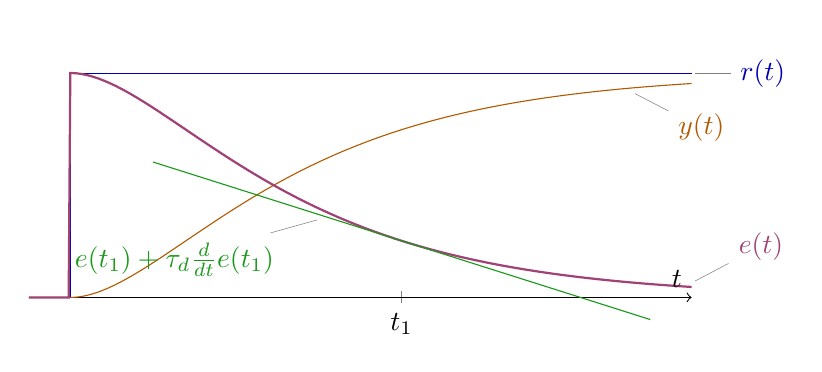
\begin{tikzpicture}
     \pgfmathdeclarefunction{overdampedresponse}{3}{%
     \pgfmathparse{1+#1/(#2-#1)*exp(-#3/#1)-#2/(#2-#1)*exp(-#3/#2)}%
     }
     \pgfmathdeclarefunction{overdampedderiv}{3}{%
     \pgfmathparse{-1/(#2-#1)*exp(-#3/#1)+1/(#2-#1)*exp(-#3/#2)}%
     }
     \pgfmathsetmacro{\tone}{2}
     \pgfmathsetmacro{\ttwo}{4}
     \pgfmathsetmacro{\xnull}{8}
     
     \pgfmathsetmacro{\enull}{1-overdampedresponse(\tone, \ttwo, \xnull)}
     \pgfmathsetmacro{\eslope}{-overdampedderiv(\tone, \ttwo, \xnull)}
     
     \begin{axis} [
     width= 10cm,
     height = 5cm,
     axis lines=middle,
     axis line style={->},
     xtick={0, \xnull},
     xticklabels={0, $t_1$},
     % ytick={0, 1},
     ytick=\empty,
     % yticklabels={0, $r_f$},
     y axis line style={draw opacity=0},
     xmin=-1,
     xmax=15,
     ymin=0,
     ymax=1.2,
     xlabel=$t$,
     clip = false,
     ]

     \addplot[solid, thin,  blue!70!black, const plot] coordinates { (-0.5, 0) (0,1) (15,1) } node[pos=0.99, pin=0:{$r(t)$},] {};
     \addplot[solid,thin, orange!70!black, domain=-1:15, samples=200] {(x>0)*(overdampedresponse(\tone,\ttwo,x))} node[pos=0.9, pin=-20:{$y(t)$},] {};
     \addplot[solid,thick, magenta!60!black, domain=-1:15, samples=400] {(x>0)*(1-overdampedresponse(\tone,\ttwo,x))} node[pos=0.99, pin=20:{$e(t)$},] {};
     \addplot[solid, ddc, domain=2:14, samples=10] {\enull + \eslope*(x - \xnull)} node[pos=0.35, pin=-160:{$e(t_1) + \tau_d\frac{d}{dt}e(t_1)$},] {};
\end{axis}  
     \end{tikzpicture}
   \end{center}

\begin{align*}
u(t) &= k_c\Big( \underbrace{\textcolor{ppc}{e(t)} + \textcolor{ddc}{\tau_d \frac{d}{dt} e(t)}}_{\text{error predicho}} + \underbrace{\textcolor{iic}{\frac{1}{\tau_i} \int_0^{t} e(\xi) d\xi}}_{\text{error acumulado}} \Big)
\end{align*}
\end{frame}

\begin{frame}[label={sec:org8b18309}]{El controlador PID en forma serial}
\begin{center}
  \begin{tikzpicture}[yscale=0.8,node distance=22mm, block/.style={rectangle, draw, minimum width=12mm}, sumnode/.style={circle, draw, inner sep=2pt},
  amp/.style = {regular polygon, regular polygon sides=3,
           draw, fill=white, text width=1em,
           inner sep=1pt, outer sep=0mm,
           shape border rotate=-90},
     ]

    \node[coordinate] (input) {};
    \node[sumnode, right of=input, node distance=16mm] (sum) {\tiny $\Sigma$};
    \node[color=iic, block, right of=sum, node distance=20mm, inner sep=3pt] (ii)  {$\frac{\tau_Is + 1}{\tau_i s}$};
    \node[color=ddc,block, right of=ii, node distance=20mm] (dd)  {$\tau_Ds + 1$};
    \node[amp, right of=dd, node distance=20mm] (gain)  {$K_c$};
    \node[coordinate, below of=sum, node distance=12mm] (feedback) {};
    \node[coordinate, right of=gain, node distance=20mm] (output) {};

    \draw[->] (input) -- node[above, pos=0.3] {$r(t)$} (sum);
    \draw[->] (sum) -- node[above, pos=0.2] {$e(t)$} node[coordinate] (mm) {}  (ii);
    \draw[->] (gain) -- node[above, near end] {$u(t)$} (output);
    \draw[->] (feedback) -- node[left, near start] {$y(t)$} node[right, pos=0.95] {-} (sum);
    \draw[->] (ii)  -- node[above,] {} (dd);
    \draw[->] (dd) -- node[above, near end] {} (gain);

  \end{tikzpicture}
\end{center}

\[F(s) = K_c \left( \frac{ \tau_I s + 1}{\tau_I s} \right) (\tau_D s + 1) 
= \underbrace{\frac{K_c(\tau_I + \tau_D)}{\tau_I}}_{k_c} \left(1 + \frac{1}{\underbrace{(\tau_I + \tau_D)}_{\tau_i} s} + \underbrace{\frac{\tau_I\tau_D}{\tau_I + \tau_D}}_{\tau_d}s \right) \]
\end{frame}
\end{document}